\documentclass[12pt, letterpaper]{article}
\usepackage[utf8]{inputenc}
\usepackage{amsmath,amsfonts,amssymb, mathtools, geometry, algorithm, algorithmic, graphicx, wrapfig, float, hyperref, array, xurl,setspace,tocloft}
\makeatletter
\renewcommand*\env@matrix[1][\arraystretch]{%
  \edef\arraystretch{#1}%
  \hskip -\arraycolsep
  \let\@ifnextchar\new@ifnextchar
  \array{*\c@MaxMatrixCols c}}
\makeatother

\geometry{margin=1in}
\doublespacing
\graphicspath{{images/}}

\begin{document}
\begin{titlepage}
    \begin{center}
       \vspace*{1cm}
       \huge
       \textbf{Modelling Constrained 2D Particle-Based Systems}\\
       \large
       \vspace{0.5cm}
        To what extent can Penalty Constraints and Relaxed Geometric Constraints model 2D particle-based constrained dynamic systems?
       \vspace{1.5cm}\\
        Subject: Math
       \vfill
        \begin{figure}[H]
        \centering
        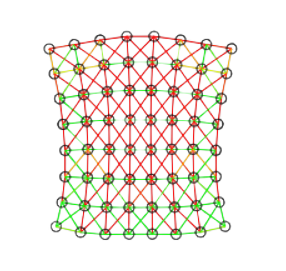
\includegraphics[width=8cm]{title clear.png}

        \end{figure} 
        \vfill
            
       \vspace{0.8cm}
     
            
       Word count: 3999\\
            
    \end{center}
\end{titlepage}


\setstretch{1.25}
%TC:ignore
\tableofcontents
%TC:endignore
\clearpage
\doublespacing

\section{Introduction}
\hspace{\parindent} Since the topic of choice is quite specific, this essay will begin with a breakdown of the research question. Constrained 2D particle-based systems comprise of a particle system and a set of constraints. Essentially, they are 2D physics simulations where the particles are ``atoms", and the constraints are ``bonds". Firstly, a particle-based system consists of a group of free-moving circles that can travel across a 2D plane. These particles (circles) have a defined radius, mass, position, velocity, and force. Moreover, particles can also interact with the surrounding given pre-defined conditions. Constraints are the pre-defined mathematical conditions that control how the particles behave, just like how a string defines the path of a pendulum. It is possible to have multiple constraints, and such systems of constraints can work together to influence the behaviour of the particles. Therefore, a constrained particle-based system is simply a set of particles that are controlled by a set of constraints. A double pendulum would be considered a constrained particle system. When visualized, systems of particles and constraints can form mesh-like objects that react under external forces $\text{(Figure 6)}$. Some examples of common constraints include bend constraints, distance constraints, and area constraints. The goal of this essay is to establish a method that applies a mathematical constraint on a set of particles such that the system can also respond to external forces. Section 2 will formally introduce the fundamental setup of the model. Later sections will generalize, compare, and analyze the effectiveness of the penalty method $\text{(Equation 23)}$ and relaxed geometric method $\text{(Equation 38)}$. Further discussions about the effectiveness of each method will also be included.

A simple programmatic implementation is provided to help visualize the mathematics within this essay ($\text{Appendix A}$). All figures are also created by the author.
%TC:ignore
\subsection{Notation}
\def\arraystretch{2}%
\begin{table}[H]
\begin{tabular}{ | m{10em} | m{11.5cm}| }
  \hline
  $x, v, a, F$ & Vector quantities: position, velocity, acceleration, and force \\ 
  \hline
  $m, r$ & Scalar quantities: mass and radius \\ 
  \hline
  $\dot{F}$ & Time derivative; equivalent to $\frac{dF}{dt}$  \\ 
    \hline
  $q_{j,i}$ & the $i^{th}$ element of $q_j$  \\ 
  \hline
  Row vector notation $\left[ x_{1}\;\; x_{2}\;\; .\; . \; .\;\;  x_{n}  \right] ^{T}$ & Equivalent to the column form, except it saves space $\begin{bmatrix}[1.1]x_{1} \\x_{2} \\ \vdots \\ x_{n}  \end{bmatrix}$ \\ 
  \hline
  $\nabla_{q_j} C_j(q_j)$ & The gradient of $C$ in terms of $q_j$, $$\begin{bmatrix} \frac{\partial}{\partial q_{j,1}} C_j(q_j)& \frac{\partial}{\partial q_{j,2}} C_j(q_j) & \cdots &  \frac{\partial}{\partial q_{j,n}} C_j(q_j)\end{bmatrix}$$ \\
  \hline
  $\nabla_{q_{j,i}}C_j(q_{j,1},x_{j,2},...x_{j,n})$ & This examines how each component of $q_{j,i}$ changes in the function $C_j$, $$\nabla_{q_{j,i}}C_j(q_{j,1},q_{j,2},...q_{j,n})$$ Looks at the specific partial derivative with respect to $q_{j,i}$
$$\frac{\partial}{\partial q_{j,i}} C_j(q_{j,1},q_{j,2}, . . ., q_{j,n})$$ \\
\hline
$x^{(k-1)}, x^{(k)}, x^{(k + 1)} $ & Shows the iterative steps of x from k-1, to k, then to k + 1\\
\hline
\end{tabular}
\centering
\caption{Explanation of prevalent notation used in the paper}
\label{table:table}
\end{table}
%TC:endignore
\clearpage

\section{Introduction to Particle-Based Systems}

\subsection{Particle Systems and Constrained Systems}
\hspace{\parindent} To keep everything consistent, the aforementioned qualities of constrained particle-systems will be mathematically abstracted in the following table.
%TC:ignore
\def\arraystretch{2}%
\begin{table}[H]
\begin{tabular}{ | m{3em} | m{13.5cm}| }
  \hline
  $p_i$ & A circular geometric object with properties $x_{i}, v_{i}, a_{i}, m_{i}, r_{i}, F_{i}$ \\ 
  \hline
  $p$ & The particle system; a concatenated list of all $n$ particle objects $[\hspace{4pt}p_{1} \hspace{4pt} p_{2} \hspace{4pt} p_{3} \hspace{4pt} \cdots \hspace{4pt} p_{n}\hspace{4pt}] ^ {T}$ (Bender) \\ 
  \hline
  $C_j$ & A single constraint function
 \begin{itemize}
  \item Defined by a function $C_j$ such that $C_{j}: \mathbb{R}^{n}\rightarrow \mathbb{R}$
  \item A function input is called a generalized property, $q_{j,i}$
  \item The set of all function inputs is called the generalized properties, $q_j$. There will always be a $q_{j,i}$ that is the stiffness factor, $k$, such that $k \in q_j$.
  \item The size of $q_j$ is $n_{j} = n(q_{j})$.
\end{itemize}
This essay will focus on time-independent constraints, where $t \notin q_{j}$ (scleronmic). Additionally, all constraints will be written as an equality, $$C_{j}(q_{j,1},q_{j,2},q_{j,3},\cdots,q_{j,n}) = 0,$$ and there will not be inequalities that results in constraint breaking (holonomic). This equation must be satisfied for the constraint to be maintained.
\\
\hline
 $C$ & the concatenated values of all $m$ different constraints $[\hspace{4pt}C_{1} \hspace{4pt} C_{2} \hspace{4pt} C_{3} \hspace{4pt} \cdots \hspace{4pt} C_{m}\hspace{4pt}] ^ {T}$\\
 \hline
\end{tabular}
\centering
\caption{Mathematical abstraction of the components in a constrained particle system}
\label{table:table}
\end{table}
%TC:endignore

\subsection{Particle System Solvers and Integration Schemes}
\hspace{\parindent} During the simulation, the constrained particle-system progresses in timesteps, $\Delta t$. This is visualized as repeated static frames of the particle system after every $\Delta t$ amount of time.
\begin{figure}[H]
\centering
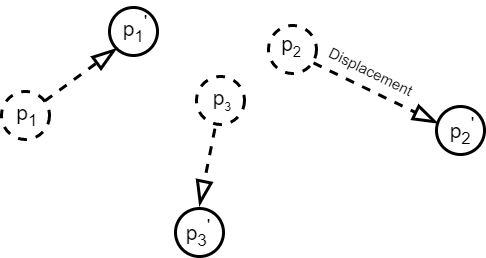
\includegraphics[width=8cm]{particle system.png}
\caption{New particle positions after $\Delta t$}
\label{fig:figure}
\end{figure} 
To find the displacements on a particle that has some velocity and some force, a set of kinematic differential equations are required. These set of equations are fundamental in physics and relate the position, velocity, and acceleration/force.  
\begin{equation}
   \begin{gathered}
        v = \dot{x}\\ 
        a = \dot{v}\\
        F = ma.
    \end{gathered} 
\end{equation}
Complex systems are solved by decomposition into a similar form as $\text{Equation 1}$. Numerical integration is then used to arrive at an approximate solution. For this paper, a predictor-corrector semi-implicit Euler integration scheme is used.

\subsubsection{Semi-Implicit Euler}
\hspace{\parindent} Semi-implicit Euler is a numerical integration method that approximates the integral of a function with an algorithmic method. This method will be used to calculate new positions of the particles. The first step of semi-implicit Euler is Euler approximation. It is an algorithm that predicts the next position from a point by extending the slope at that point by a predefined step $\text{(Figure 2)}$. 
\begin{figure}[H]
    \centering
    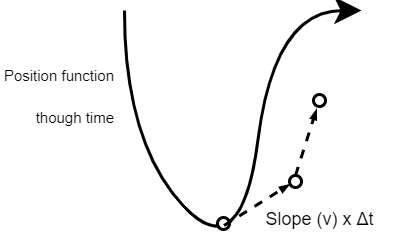
\includegraphics[width=7cm]{euler.png}
    \caption{Visualization of Euler algorithm}
    \label{fig:my_label}
\end{figure}
\noindent Compared to normal Euler, semi-implicit Euler first completes the Euler step on velocity then uses that new value to approximate the position. According to Equations 1, the slope of a velocity vs. time curve is the acceleration, $a$. And the slope of a position vs. time curve is the velocity, $v$. Therefore,
\begin{equation}
    \begin{gathered}
        v^{(k+1)}= v^{(k)} + a^{(k)}\Delta t \\
        x^{(k+1)}= x^{(k)} + v^{(k + 1)}\Delta t,
    \end{gathered}
\end{equation}
and when combined, 
\begin{equation}
    x^{(k+1)} = x^{(k)} + v^{(k)}\Delta t + a^{(k)}\Delta t^{2}.
\end{equation}
Implicit integration schemes solve the system both at the current time and at a future time. Typically, implicit algorithms are much more stable. At a glance, Equations 2 seem explicit as the system is solved for the future position $x^{(k+1)}$ after $\Delta t$. This is not entirely true as the velocity of the current system must be solved first, and that solved result is used to determine the new position. For lower values of $\Delta t$, error decreases notably and the system is stable like  implicit methods. Whereas for larger values of $\Delta t$, the system becomes unstable like explicit methods $\text{(Liu)}$. Because of this behaviour, this method is described as semi-implicit in literature. 

The traditional Euler algorithm has an error value of $O(\Delta t^{2})$ $\text{(Fitzpatrick)}$, which is the truncation error of the algorithm. Since it only accounts for acceleration, any higher derivatives (jerk, crackle, pop) are truncated as an error. Because semi-implcit Euler is a degree higher, its corresponding error will be $O(\Delta t^{3})$ $\text{(Liu)}$. 

\subsubsection{Predictor-Corrector}
\hspace{\parindent} Predictor-Corrector is an algorithmic enhancement that makes semi-implicit Euler more stable. Predictor-Corrector finds the corrective position displacements based on a predicted future position, then directly calculates the final velocity impulse with the previous position $\text{(Figure 3)}$. 
\begin{figure}[H]
\centering
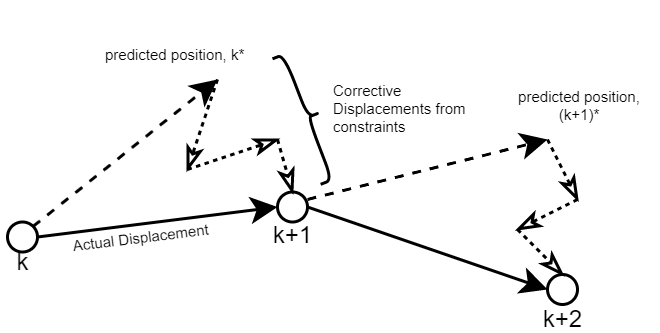
\includegraphics[width=13cm]{predictor.png}
\caption{The predictor-corrector model over 3 iterations}
\label{fig:figure}
\end{figure}
\noindent To calculate the predicted position $x*$,
$$x^{*} =  x^{(k)}  + v^{(k)}\Delta t + a^{(k)}\Delta t^{2}.$$
Then applying the corrective displacement, $\Delta x^{(k)}$, on $x*$,
$$x^{(k + 1)} = x^{*} + \Delta x^{(k)}.$$
The final velocity of the particle can be found using $v = \frac{\Delta x}{\Delta t}$,
\begin{equation}
    v^{(k+1)} = \frac{x^{(k + 1)} - x^{(k)}}{\Delta t}.
\end{equation}
Clavet's paper verifies the efficacy of the Predictor-Corrector model in resolving most overshoot problems caused by extreme forces in the semi-implicit Euler algorithm.

\subsubsection{Iterative Gauss-Seidel}
\hspace{\parindent} The previous sections discuss how the new positions of a single particle is calculated. To find the set of all displacements, $\Delta x$, that solve the particle system, $p$, a Gauss-Seidel-like local iterative solver is used. Local iterative solvers converge to the global solution by repeatedly calculating the local $\Delta x_i$ for each $p_i \in p$. Local iterative solvers are generally easier to implement and faster to compute $\text{(Jakobsen)}$.

Gauss-Seidel is a divide-and-conquer algorithm that finds the approximate solution by repeatedly solving simpler counterparts. Since most constraint systems are nonlinear, an iterative ``Gauss-Seidelization" $\text{(Gutiérrez)}$ of the Gauss-Seidel algorithm is used. For a system of constraints $\phi$, this is represented mathematically as,
\begin{equation}
    \begin{gathered}
        x_{1} ^{(k + 1)} = \phi_{1}(x_{1}^{(k)},x_{2}^{(k)}, . . ., x_{n}^{(k)} )\\
        x_{2} ^{(k + 1)} = \phi_{2}(x_{1}^{(k + 1)},x_{2}^{(k)}, . . ., x_{n}^{(k)} )\\
        \vdots\\
        x_{n} ^{(k + 1)} = \phi_{n}(x_{1}^{(k + 1)},x_{2}^{(k + 1)}, . . ., x_{n}^{(k + 1)} ).
    \end{gathered}
\end{equation}
The system of $\phi$ is lower triangular, with the bottom below the diagonal being $k + 1$ and the rest being $k$ iterations. In practice, this behaves as if the system updates after each constraint is solved; the updated value of the solved constraints are used to solve the next constraints. For a linear system, the rate convergence can be calculated with the spectral radius, $\rho = (cos \frac{\pi}{\epsilon + 1})^{2}$ $\text{(Strang)}$. Where $\epsilon$ is the number of elements in the vector $\Delta x$, and hence, the number of constraints. Generally, for $k$ iterations, the error is multiplied by $\rho ^{k}$ $\text{(Strang)}$. Admittedly, this concept is untrue for non-linear systems, but it can still approximate the expected rate of convergence. As such, the convergence rate also decreases for non-linear systems as $\epsilon$ increases. However, Gauss-Seidel can also diverge under certain conditions. ($\text{Detailed analysis will be available in Sections 3.3.2 and 4.3.2}$)

\subsection{General Solver Algorithm}
Combining all of the previous components create a general solver algorithm. Elements of this solver are influenced by Clavet’s paper. Although this essay explicitly focuses on the constraint component, other rudimentary features such as collision handling are included for an enhanced user experience. $\text{(Code available in Appendix A)}$
%TC:ignore
\begin{algorithm}[H]
\caption{General system solver for constrained particle-based systems}
\begin{algorithmic}[1]
\STATE // Run solver for every frame
\LOOP 
    \STATE // Iterate iterationNumberPerFrame times per frame
    \FOR{$k \leftarrow 0$ \textbf{to} $iterationNumberPerFrame$}
        \FORALL{$p_{i} \in p$}
            \STATE // Update velocity with gravity
            \STATE $v_{i} \leftarrow v_{i} + g\Delta t$
            \STATE // Update velocity with other external forces
            \STATE $v_{i} \leftarrow F_{i}/m_{i} \cdot \Delta t$
            \STATE //Save current position to previous position
            \STATE $x_{i}^{prev} \leftarrow x_{i}$
            \STATE // Move to predicted position, x*
            \STATE $x_{i} \leftarrow x_{i} + v_{i}\Delta t$
        \ENDFOR
        \STATE // Algorithm 2, Section 3.3
        \STATE applyPenaltyConstraints()
        \STATE // Algorithm 3, Section 4.3
        \STATE applyRelaxedConstraints()
        \STATE // Additional functions for improved user experience
        \STATE resolveParticleInterations()
        \STATE resolveCollisions()
        \STATE // Equation 3: calculate the velocity
        \FORALL{$p_{i} \in p$}
            \STATE $v_{i} \leftarrow (x_{i} - x_{i}^{prev})/\Delta t$
        \ENDFOR
    \ENDFOR
\ENDLOOP
\end{algorithmic}
\end{algorithm}
%TC:endignore
\section{Penalty Constraints (PC)}
\subsection{Explanation and Generalization}


\hspace{\parindent} Penalty constraints are a type of constraints that can be used in constrained particle systems. In essence, PCs treat all constraints as springs. This means that any deviation from $C(q) = 0$ will cause a penalty force in the opposite direction of the displacement, just like a spring $\text{(Figure 4)}$. 
\begin{figure}[H]
\centering
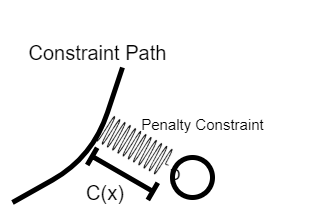
\includegraphics[width=6.5cm]{pc.png}
\caption{Penalty Constraint Visualization}
\label{fig:figure}
\end{figure} 
The spring-like behaviour can be described using Hooke's law,
\begin{equation}
    F = -k \Delta s.
\end{equation}
Where $k$ is the spring constant that determines how stiff a spring is, and $\Delta s$ is how much the spring is displaced. However, this system has an obvious problem: penalty forces can increase greatly for stiff systems with higher spring constants. The excessive force impulses create large corrective displacements, and when combined with the error of semi-implicit Euler (Section 2.2.1), can cause the system to quickly become unstable. 

As an example, Hooke's law will be geometrically applied on a distance constraint, where a pair of constrained particles must be a certain distance apart. Let two particles be constrained by length, r, as shown in Figure 5.
\begin{figure}[H]
\centering
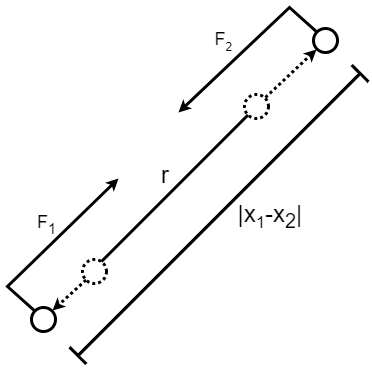
\includegraphics[width=7cm]{pc diagram.png}
\caption{Distance constraint with the PC method}
\label{fig:figure}
\end{figure} 
\noindent Given $F = -k\Delta s$,
\begin{equation}
    \begin{gathered}
        F_{1}=-k(|x_{1}-x_{2}|-r)\frac{x_{1}-x_{2}}{|x_{1}-x_{2}|}\\
        F_{2}=k(|x_{1}-x_{2}|-r)\frac{x_{1}-x_{2}}{|x_{1}-x_{2}|},
    \end{gathered}
\end{equation}
 where $\Delta s = |x_{1} - x_{2}| - r$, and $\frac{x_{1} - x_{2}}{|x_{1} - x_{2}|}$ is the direction unit vector. Although the geometric intuition works, it is not sufficient. Next, a generalization of the penalty method will be attempted. 

Assuming that the constraints behave as springs, it is possible to calculate the energy that the constraint holds, much like a real spring. The value of this potential energy can then be used to calculate the force applied on each particle, hence resulting in some displacement. 
Let a constraint be $C_j(x_{1},x_{2},x_{3}, . . . , x_{n}, k) = 0$, where $x_i$ is the position of particle $p_i$. Similarly, the generalized properties will be $q_j = [\hspace{4pt}x_{1} \hspace{4pt} x_{2} \hspace{4pt} \cdots \hspace{4pt} x_{n}\hspace{4pt}\hspace{4pt} k] ^ {T}$. Then Hooke's law can be used to calculate the penalty forces for the constraint. Because the equilibrium position is $C_j(q_j) = 0$, the deviation will be $ \Delta s = C_j(q_j)$. Therefore, the force will be $F_{C_j} = -kC_j$.

In physics, energy is defined as 
$$E= \intop_{s_i}^{s_f}  F\cdot ds,$$
where $[s_i, s_f]$ is the interval of displacement that the force $F$ is applied. Consequently, the force for a penalty constraint will be applied on the displacement interval $[0, C_j]$. Then the energy function of constraint $C_j$ will be, 
$$E_{C_j}=\intop_{0}^{C_j}  F_{C_j}\cdot dC_j$$
Using $F_{C_j} = -kC_j$,
$$E_{C_j} = \intop_{0}^{C_j} -kC_j \cdot dC_j$$
$$= \left. -\frac{1}{2}kC_j\cdot C_j \right|_{0}^{C_j} =  -\frac{1}{2}kC_j\cdot C_j -0$$
\begin{equation}
   E_{C_j}= -\frac{1}{2}kC_j\cdot C_j.
\end{equation}
Conversely, the force and energy is related by the formula
\begin{equation}
   F_{x} = \frac{\partial E}{\partial x}.
\end{equation}
Therefore, the force affecting each particle position, $x_i$, will be
\begin{equation}
   F_{x_{i}} = \frac{\partial E_{C_{j}}}{\partial x_{i}}.
\end{equation}
This can be simplified further by substituting in $\text{Equation 8}$,
\begin{equation}
    F_{x_{i}} = C_j\cdot \frac{\partial C_j}{\partial x_{i}}.
\end{equation}
Because of the predictor-corrector model (Section 2.2.2), a corrective displacement from the resulting force must be calculated. To do so, the acceleration is first calculated with Newton’s Second law, $F = ma$. Rearranging yields, $$a = m_i^{-1}F_{x_i}.$$ 
The next step involves discretizing the acceleration, $a$. Discretization uses the semi-implicit Euler algorithm (Section 2.2.1) to convert $a$ into $\Delta x$. Recall, 
$$x^{(k+1)} = x^{(k)} + v^{(k)}\Delta t + a^{(k)}\Delta t^{2}.$$
Then,
$$\Delta x^{(k)} = x^{(k+1)} - x^{(k)}$$
$$\Delta x^{(k)} = v^{(k)}\Delta t + a^{(k)}\Delta t^{2}.$$
In the predictor-corrector model, each corrective displacement caused by a force is independent of the particle velocity. Therefore,
$$\Delta x = a^{(k)}\Delta t^{2}.$$
Using the result from Newton's Second Law, 
\begin{equation}
   \Delta x = w_i F_{x_i}\Delta t^{2}.
\end{equation}
where $w_i$ is the inverse mass $m_i^{-1}$. Then substituting with $\text{Equation 11}$ yields,
\begin{equation}
    \Delta x_{i} = -w_{i}kC_j\cdot \frac{\partial C_j}{\partial x_{i}} \Delta t^{2}.
\end{equation}
To verify the derived formula, it will be applied to the case example stated in Figure 5. The mathematical representation of the distance constraint will be
\begin{equation}
    C_j(x_{1},x_{2}, k) = |x_{1}-x_{2}|-r.
\end{equation}
This constraint maintains a distance $r$ from two particles with positions $x_1$ and $x_2$.
Using Equation 11, the penalty forces for each $x$ are
\begin{equation}
    \begin{gathered}
        F_{x_{1}}=-k(|x_{1}-x_{2}|-r)\frac{x_{1}-x_{2}}{|x_{1}-x_{2}|}\\
        F_{x_{2}}= k(|x_{1}-x_{2}|-r)\frac{x_{1}-x_{2}}{|x_{1}-x_{2}|}.
    \end{gathered}
\end{equation}
These results match the intuitive geometric results calculated earlier. This can be taken a step further with the discretization in Equation 13, of which
\begin{equation}
    \begin{gathered}
        \Delta x_{1}=-w_{1}k(|x_{1}-x_{2}|-r)\frac{x_{1}-x_{2}}{|x_{1}-x_{2}|} \Delta t^{2}\\
        \Delta x_{2}=w_{2}k(|x_{1}-x_{2}|-r)\frac{x_{1}-x_{2}}{|x_{1}-x_{2}|} \Delta t^{2}.
    \end{gathered}
\end{equation}
(Detailed derivation available in Appendix B)


\subsection{Damping}
\hspace{\parindent} Another major part of PCs is damping. Much like in real life, springs are affected by internal frictional forces that causes them to lose energy with time. This artificially induced energy loss can help prevent the system from becoming unstable. Typically, a damping force, $D_j$, is proportional to the velocity $\text{(Adams)}$. Since this is the damping for a constraint, the respective velocity will be of the constraint itself (the rate of which the constraint contracts/extends). This is denoted mathematically as $v_{C_j} = \dot{C_j}$. Hence, $D_j$ can be rewritten with an arbitrary damping constant, $\mu$, as
\begin{equation}
    D_j =  \mu \dot{C_j}.
\end{equation}
Next, to calculate how the constraint will behave with damping, the penalty forces with damping must be derived. Similar to Section 3.1, a potential energy function will be required.\\
Let the function $F_{C_j} = -kC_j - D_j$, where $-kC_j$ is the force of the constraint and $- D_j$ is the damping force opposing the constraint (hence the negative), and by calculating the corresponding energy function, 
$$E_{C_j} =  \intop_{0}^{C_j} F_{C_j} \cdot dC_j =  \intop_{0}^{C_j} (-kC_j - \mu \dot{C_j}) \cdot dC_j.$$
Expanding the integral gives
$$=  \intop_{0}^{C_j} -kC_j \cdot dC_j -  \intop_{0}^{C_j} \mu \dot{C_j} \cdot dC_j$$
$$=  \intop_{0}^{C_j} -kC_j \cdot dC_j -  \intop_{0}^{C_j} \mu \frac{d C_j}{d t} \cdot dC_j,$$
and by evaluating,
$$= \left. -\frac{1}{2}kC_j\cdot C_j \right|_{0}^{C_j} - \left. \mu \frac{d C_j}{d t} \cdot C_j \right|_{0}^{C_j}$$
\begin{equation}
   E_{C_j} = - \frac{1}{2} k C_j \cdot C_j - \mu \frac{d C_j}{d t} \cdot C_j. 
\end{equation}
Now the individual forces can be found from Equation 18, the energy function. Recall Equation 11, 
\begin{equation*}
    F_{x_{i}} = \frac{\partial E}{\partial x_{i}}.
\end{equation*}
Therefore,
$$F_{x_{i}} = \frac{\partial}{\partial x_{i}} \left( - \frac{1}{2} k C_j \cdot C_j - \mu \frac{d C_j}{d t} \cdot C_j \right)$$
\begin{equation}
    =\frac{\partial}{\partial x_{i}}\left( -\frac{1}{2} k C_j \cdot C_j \right) - \frac{\partial}{\partial x_{i}} \left(\mu \frac{d C_j}{d t} \cdot C_j \right).
\end{equation}
Next, the end term $\frac{\partial}{\partial x_{i}} (\mu \frac{d C_j}{d t} \cdot C_j)$ can be broken down with the product rule to
$$\mu \left( \frac{\partial}{\partial x_{i}} \frac{dC_j}{dt} \cdot C_j + \frac{dC_j}{dt} \cdot \frac{\partial C_j}{\partial x_{i}} \right).$$
Performing a swap and factor then yields
$$\mu \left(\frac{d}{dt} \frac{\partial C_j}{\partial x_{i}}  \cdot C_j + \frac{dC_j}{dt} \cdot \frac{\partial C_j}{\partial x_{i}} \right) = \mu  \frac{\partial C_j}{\partial x_{i}} \left(\frac{d}{dt} \cdot C_j + \frac{dC_j}{dt}\right). $$
Finally simplifying to
\begin{equation}
    2 \mu \frac{\partial C_j}{\partial x_{i}} \cdot \frac{dC_j}{dt}.
\end{equation}
Now, substituting back and continuing with Equation 19 gives

$$F_{x_{i}} = -kC_j \cdot \frac{\partial C_j}{\partial x_{i}} - 2 \mu \frac{\partial C_j}{\partial x_{i}} \cdot \frac{dC_j}{dt}$$
\begin{equation}
     F_{x_{i}} = \left(-kC_j - 2\mu \frac{d C_j}{d t}\right)\cdot \frac{\partial C_j}{\partial x_{i}},
\end{equation}
and because $\mu$ is an arbitrary damping constant, $2\mu$ can be condensed into $\mu$. Further simplification yields similar results as Witkin, where
\begin{equation}
    F_{x_{i}} = (-kC_j - \mu \dot{C_j}) \cdot \frac{\partial C_j}{\partial x_{i}}.
\end{equation}

Lastly, using the previous method, the force from Equation 22 is discretized to calculate the position.
Given $a_{i} = w_{i}F_{x_{i}}$ and $\Delta x_{i} = a_{i}  \Delta t ^{2}$, then
\begin{equation}
    \Delta x_{i} = w_{i}(-kC_j - \mu \dot{C_j}) \cdot \frac{\partial C_j}{\partial x_{i}} \Delta t^{2}.
\end{equation}
Equation 23 is the final equation for penalty constraints, which take into account damping. When the damping constant is 0, Equation 23 decomposes into Equation 13. Once again, applying the results on the constraint function $C_j(x_{1},x_{2}) = |x_{1}-x_{2}|-r$ yields the new set of equations,
\begin{equation}
    \begin{gathered}
        \Delta x_{1} = w_{1}\left(-k(|x_{1}-x_{2}|-r) - \mu \frac{(v_{1} - v_{2}) \cdot (x_{1} - x_{2})}{|x_{1}-x_{2}|}\right) \cdot \frac{x_{1}-x_{2}}{|x_{1}-x_{2}|} \Delta t^{2}\\
        \Delta x_{2} = -w_{2}\left(-k(|x_{1}-x_{2}|-r) - \mu \frac{(v_{1} - v_{2}) \cdot (x_{1} - x_{2})}{|x_{1}-x_{2}|}\right) \cdot \frac{x_{1}-x_{2}}{|x_{1}-x_{2}|} \Delta t^{2}.
    \end{gathered}
\end{equation}
$\text{(Detailed derivation available in Appendix B)}$

\subsection{Programmatic Implementation and Analysis}
\hspace{\parindent} For later analysis and mathematical verification, Equations 24 are implemented programmatically. $\text{(Code and demonstration available in Appendix A)}$
\begin{algorithm}[H]
\caption{Penalty Constraint Algorithm - applyPenaltyConstraints()}
%TC:ignore
\begin{algorithmic}[1]
\STATE //loop through all constraint solving iterations
\FOR{$k \leftarrow 0 \hspace{4pt} \textbf{to}$ constraintSolvingIterationNumber}
    \STATE //Iterative Gauss-Seidel step for each constraint
    \FORALL{$C_{j} \in C$}
        \STATE // Calculate Penalty Forces
        \STATE $force \leftarrow calculateForce()$
        \STATE //Discretize force to find displacement
        \STATE $\Delta x \leftarrow force \cdot \Delta t$
        \STATE // Apply displacement
        \STATE $x \leftarrow x + \Delta x$
    \ENDFOR
\ENDFOR
\end{algorithmic}
\end{algorithm}
%TC:endignore

\subsubsection{Inconsistent Stiffness}
\hspace{\parindent} Inconsistent stiffness is the first problem with the iterative Gauss-Seidel algorithm (Section 2.2.3). As described in Algorithm 1, the $iterationNumberPerFrame$ can be increased to solve the system multiple times every frame. Increasing the $iterationNumberPerFrame$ can speed up system convergence as the error is multiplied by $p^k$, where $k$ is the iteration number $\text{(Section 2.2.3)}$. Unfortunately, speeding up system convergence also alters constraint stiffness $\text{(Macklin)}$. This dependence results in arbitrary stiffness units, resulting in an unsuitable method for realistic physical modelling. To negate this issue, the iterative solver can be replaced with a global solver that directly computes the solution, which ignores any convergence errors $\text{(Witkin)}$.
\begin{figure}[H]
\centering
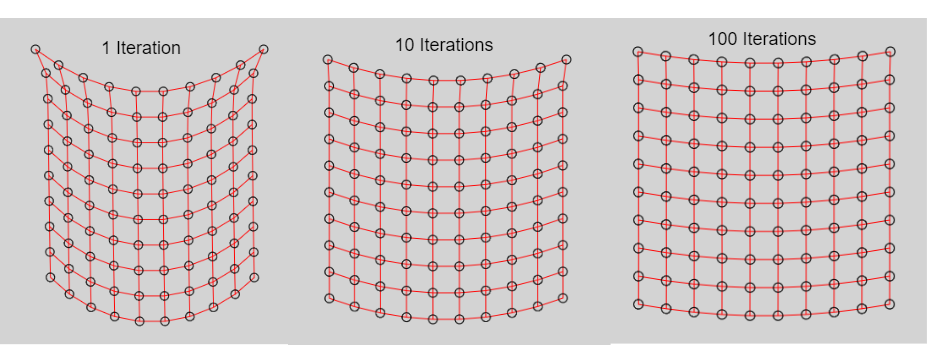
\includegraphics[width=14cm]{pc stiffness.png}
\caption{PC stiffness behaviour for different iterations (the uniform red colour is due to the high forces on the constraints with a stiffness of 100000)}
\label{fig:figure}
\end{figure} 
It is observed in Figure 6 that more iterations result in higher stiffness. This is because the convergence error from the Gauss-Seidel algorithm is reduced with more iterations. More iterations also cause constraint penalty force displacements to multiply, behaving as if it was a larger displacement caused by larger stiffness $\text{(Figure 7)}$.
\begin{figure}[H]
\centering
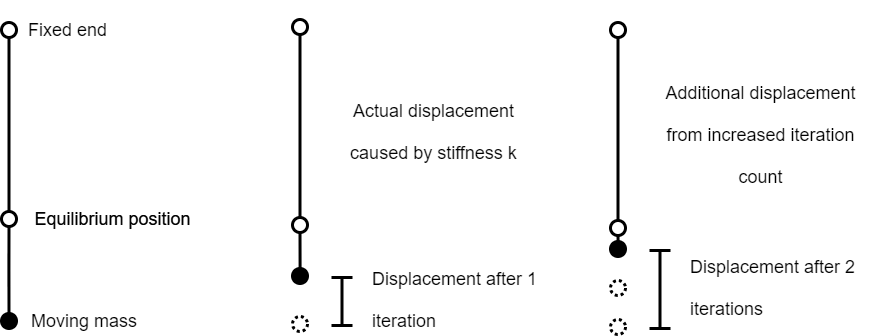
\includegraphics[width=15cm]{pc stiffness exp 1.png}
\caption{Increased PC stiffness with iteration number}
\label{fig:figure}
\end{figure} 
\noindent However, using $iterationNumberPerFrame$ as a means to increase stiffness can be more stable than simply increasing $k$. Smaller iterative steps can help combat overshoot for large stiffness values, as demonstrated in Figure 8. 
\begin{figure}[H]
\centering
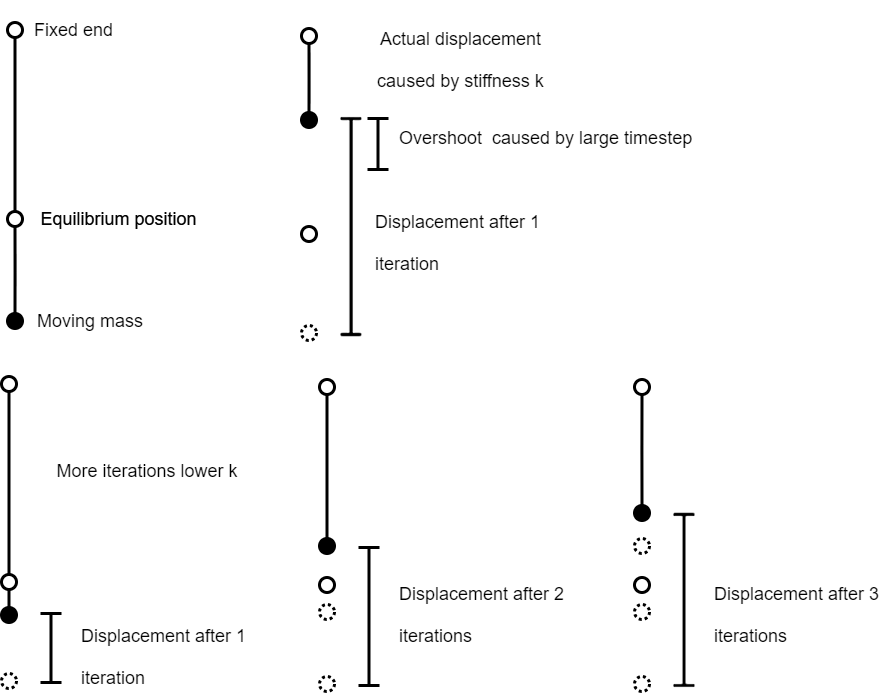
\includegraphics[width=15cm]{pc stiffness exp 2.png}
\caption{Induced PC stiffness stability for increased iteration number}
\label{fig:figure}
\end{figure} 
\noindent For effective rigid systems, it is important to find an empirical balance of $k$, $\Delta t$, and $iterationNumberPerFrame$.

\subsubsection{Convergence and Energy Conservation}
\hspace{\parindent} Convergence and energy conservation are also key concepts of physical modelling. Inconsistencies in the energy conservation could result in unrealistic physical models. Ideal PCs do not converge; instead, they oscillate like a spring between different stable states about $C(q) = 0$ $\text{(Goldstein)}$. Just like how a pendulum will stay forever swinging without energy loss, convergence to a static equilibrium is only induced when damping causes a energy loss within the system.
\begin{figure}[H]
\centering
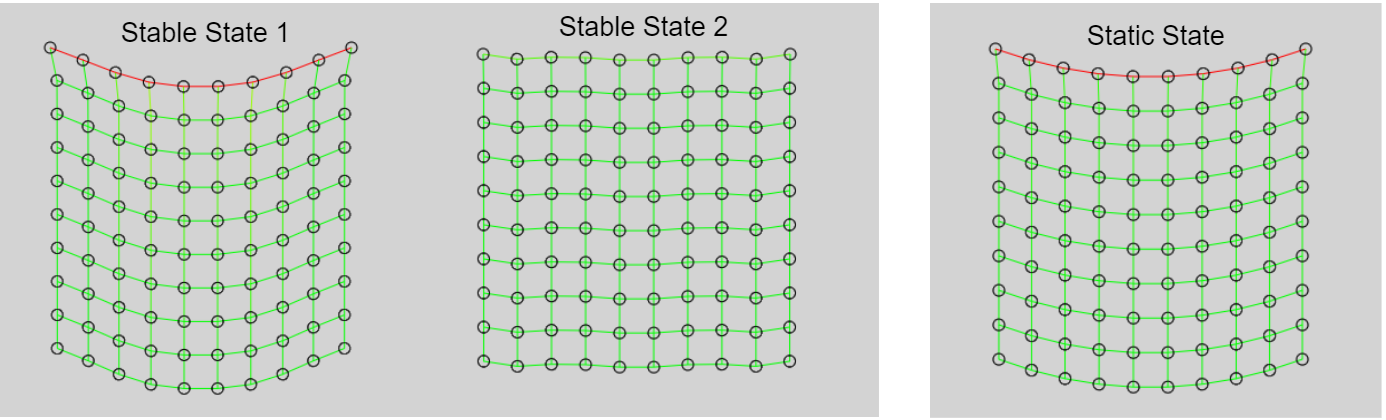
\includegraphics[width=14cm]{pc stable-static.png}
\caption{Stable oscillatory behaviour vs convergent behaviour}
\label{fig:figure}
\end{figure} 
\noindent Overall system convergence is dependent on the Gauss-Seidel solver. Generally, the larger the system, the longer it takes to converge. As discussed in Section 2.2.3, increasing the \\$iterationNumberPerFrame$ increases the system convergence rate. However, ideal systems with no damping still seem to lose energy with time, with the rate being influenced by $\Delta t$. Increasing $\Delta t$ increases the error from the semi-implicit Euler algorithm by $O(\Delta t^3)$ ($\text{Section 2.2.1}$). The truncated error behaves as an energy deficit and leads to faster energy loss. Similarly, if the system is large, individual constraint errors will accumulate, leading to greater energy dissipation. Larger penalty forces can also induce greater errors during the force discretization, $\Delta x_i = w_i F_i \Delta t^2 $ (of which $\Delta t$ also plays a role). This issue is verified with a simple pendulum simulation. The graphs in Figure 10 represent the y-position of the swinging mass through time. $\text{(Raw data available in Appendix A)}$
\begin{figure}[H]
\centering
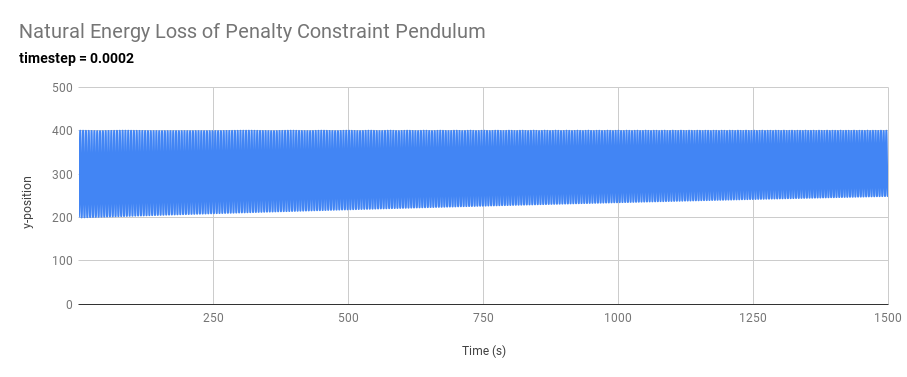
\includegraphics[width=16cm]{pc pendulum 2.png}
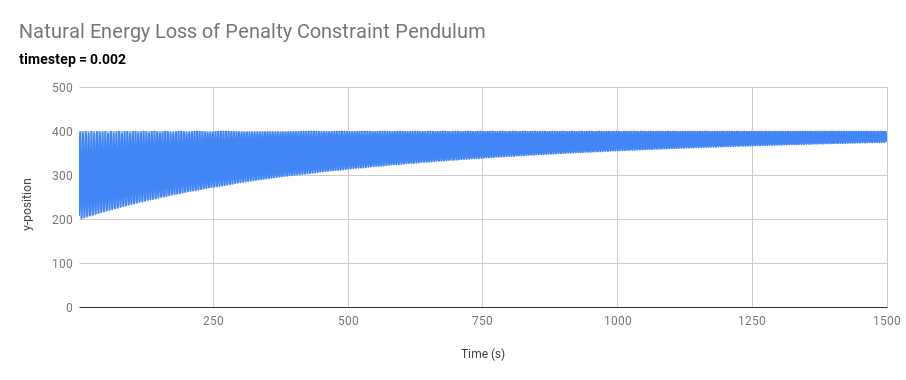
\includegraphics[width = 16cm]{pc pendulum 1.png}
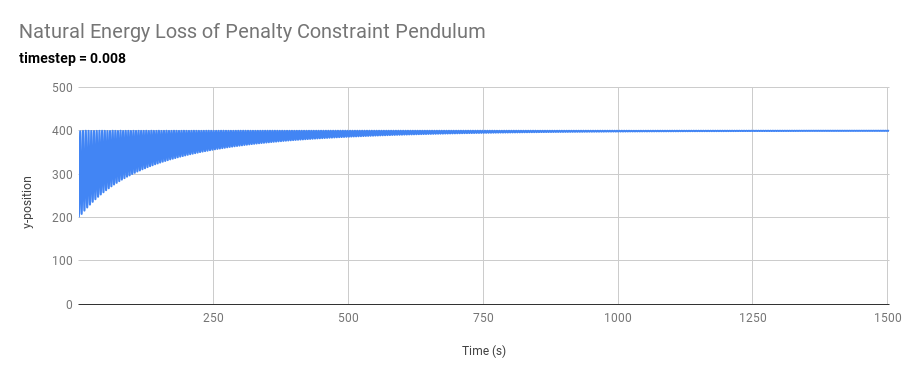
\includegraphics[width = 16cm]{pc pendulum 3.png}
\caption{y-position vs time graphs of PC pendulum systems for different $\Delta t$}
\label{fig:figure}
\end{figure} 
\clearpage
In contrast, systems can also be unstable and divergent, where the system gains energy and explodes out of control. 
\begin{figure}[H]
\centering
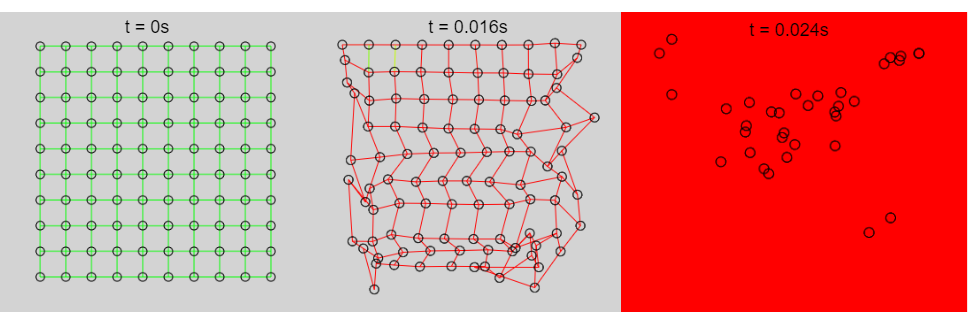
\includegraphics[width=13cm]{pc diverge dt = .008.png}
\caption{PC divergence at $\Delta t = 0.008$}
\label{fig:figure}
\end{figure} 
\noindent Divergent behaviour is caused by overestimation from the semi-implicit Euler algorithm. Divergence can be resisted with the inclusion of damping, where damping provides a buffer for overshoot. Moreover, divergence can be minimized by increasing the iteration count while lowering the forces (ex. gravity, k), or decreasing $\Delta t$.

\section{Relaxed Geometric Constraints (RGC)}
\subsection{Explanation and Generalization}
\hspace{\parindent} RGCs approximate the true constraint path by solving the constraint geometrically. Visually, it skips all the energy derivations and it appears that the ``tense” constraint is moved (relaxed) to its ideal form. The ``relaxation" of this method refers to the projection of the current positions to the next closest legal positions such that the constraint function is satisfied. Once again, a straightforward geometric derivation of a simple case is presented below in Figure 12. 
\begin{figure}[H]
\centering
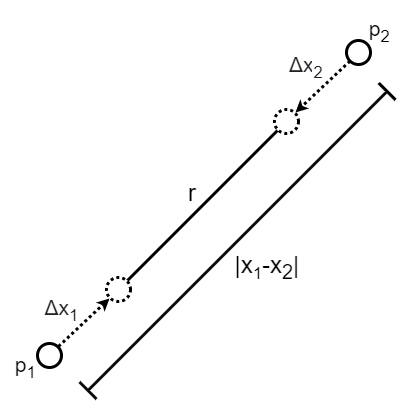
\includegraphics[width=7cm]{rgc diagram.png}
\caption{RGC Stretch Constraint}
\label{fig:figure}
\end{figure} 
\noindent Where $r$ is the ideal length and $|x_{1}-x_{2}|$ is the current length.
If $p_1$ and $p_2$ have the same mass, both will move the same amount to reach the ideal position. 
Therefore, $$|\Delta x_{1}| = |\Delta x_{2}| = \frac{1}{2} (|x_{1}-x_{2}| - r).$$
Intuitively, the contraction will be collinear with $x_1-x_2$. Hence, the final contraction must be scaled with the directional unit vector,
\begin{equation}
    \begin{gathered}
        \Delta x_{1} = -\frac{1}{2} (|x_{1}-x_{2}| - r) \frac{x_{1} - x_{2}}{|x_{1} - x_{2}|}\\
        \Delta x_{2} = \frac{1}{2} (|x_{1}-x_{2}| - r) \frac{x_{1} - x_{2}}{|x_{1} - x_{2}|}.
    \end{gathered}
\end{equation}
Equations 23 will be verified later with rigorous mathematical derivation. For now, it provides a general idea of RGCs. 

As previously mentioned, RGCs are purely position-based (ignores force and energy), which offers more control. But as a result, extra caution is needed to conserve realistic physical meaning. For an accurate physical model, the system’s linear momentum and angular momentum must be conserved. In physics, this is represented by 
\begin{equation}
    \sum\limits_{i}^{n} m_{i} \Delta x_{i} \; \;  
    \text{and} \; \; \sum\limits_{i}^{n} r_{i} \times \Delta x_{i}.
\end{equation}
Where $r_{i}$ is the distance to some common rotation center of the whole particle system and $x_i$ is the position value of a particle, $p_i$. They will be useful for providing the necessary information to calculate the final relaxation. The RGC process begins by setting up the system to be solved for a single constraint $C_j$, which is
\begin{equation*}
    \begin{gathered}
        q'_{j,1} = q_{j,1} + \Delta q_{j,1}\\
        q'_{j,2} = q_{j,2} + \Delta q_{j,2}\\
        \vdots\\
        q'_{j,n} = q_{j,n} + \Delta q_{j,n},
    \end{gathered}
\end{equation*}
such that each $\Delta q_j$ moves $q_j$ into a legal position for $C_j$,
\begin{equation}
    C_j(q_{j}) = 0 \; \; \text{and} \; \; C_j(q_{j} + \Delta q_{j}) = 0.
\end{equation}

The goal for a constraint $C_j$ is to calculate $\Delta q_j$ to find $q_j + \Delta q_j$. The set of $q_j$ can be specified further because some values $q_{j,i} \in q_j$, do not change. Namely, the mass and radius of each particle will remain constant, hence they will not need to be solved for. For this essay, the only changing values of particle $p_i$ will only be the position, $x_i$ ($v, a, F$ are disregarded because RGCs are position based).  Therefore, the list $q_j$ can be further simplified into $q_j = [x_a\;\;x_b\;\;x_c\;\;...\;]^T.$ Where $x$ is the list of all positions $[x_1 \;x_2 \; ...\;x_n]$, and $x_a,x_b,x_c\;... \in x$. Solving for $\Delta q_j$ is difficult because $C_j$ is a nonlinear function, so $C_j$ is first approximated using local linearization $\text{(Bender)}$. This method is an extension of Newton's method of finding roots. Newton's method states for a initial point $x_0$, displacement $h$, and function $f(x)$,
$$f(x_0 + h) = f(x_0) + hf'(x_0) + O(h^2).$$
The vector-valued function equivalent of $f'(x_0)$ is the gradient $\nabla_{x_0} C(x_0)$, which essentially describes the slope of $C(x_0)$ at the point $x_0$. And with $f(x) = C_j(q_j)$ and $h = \Delta q_j$,
\begin{equation}
    C_j(q_j + \Delta q_j) = C_j(q_j) + \nabla_{(q_j)}C(q_j) \cdot \Delta x + O(\Delta q_j^{2}) = 0.
\end{equation}
The error term $O(\Delta q_j^{2})$ is caused by the truncation of higher degree derivatives, much like Euler's algorithm in Section 2.2.1. The erroneous displacements resulting from this error leads to energy loss and inaccurate results. To simplify the equation, the error term can be ignored, resulting in an approximation of
\begin{equation}
    C_j(q_j) + \nabla_{q_j} C_j(q_j)^{T} \cdot \Delta q_j \approx 0.
\end{equation}
Equation 29 needs to be solved to find $\Delta q_j$, but it is currently underdetermined. This indicates there must be another relationship of $\Delta q_j$. The previously discussed conservation of linear momentum $\text{(Equation 26)}$ can be used to limit the possible values of $\Delta q_j$. Using the conservation of linear momentum, $\Delta q_j$ must be in the same direction as  $\nabla_{q_j}C_j(q_j)$ or else extra directions will be introduced. Therefore, $\Delta q_j$ will be a scalar multiple of the vector $\nabla_{q_j}C_j(q_j)$. Now, $\Delta q_j$ is rewritten as
\begin{equation}
   \Delta q_j = \lambda \nabla_{q_j}C_j(q_j)^{T}.
\end{equation}
Where $\lambda$ is the extension factor (relaxation factor). However, the above relationship for $\Delta q_j$ is only true for particles of same mass. When different masses are introduced, the scaling will be different as massive particles are harder to move compared to lighter particles. The next step will calculate the mass-scaling relationship from the laws of conservation of momentum. Recall, 
$$\sum\limits_{i}^{n} m_{i} \Delta x_{i} = 0.$$
Systems with constant mass, $m$, behave such that,
$$\sum\limits_{i}^{n} m \Delta x_{i} = 0.$$
Dividing both sides by $m$,
$$\sum\limits_{i}^{n} \Delta x_{i} = 0.$$
To achieve the same effect for a system with different masses, each $\Delta x_{i}$ is multiplied with its reciprocal mass $1/m_{i}$ (denoted as $w_{i}$) of that same particle $p_i$,
\begin{equation}
    \sum\limits_{i}^{n} m_{i}\frac{1}{m_{i}} \cdot \Delta x_{i} = 0 \rightarrow \sum\limits_{i}^{n} \Delta x_{i} = 0.
\end{equation}
Similarly, for angular momentum,
\begin{equation}
   \sum\limits_{i}^{n} r_{i} \times (m_{i}\frac{1}{m_{i}} \cdot \Delta x_{i}) = 0 \rightarrow \sum\limits_{i}^{n} r_{i} \times \Delta x_{i} = 0. 
\end{equation}
And because $q_j \in x$, 
$$
   \sum\limits_{i}^{n} \Delta q_{j,i} = 0 \text{ and } \sum\limits_{i}^{n} r_{i} \times \Delta q_{j,i} = 0
$$
Hence Equation 32 can be modified to include the mass scaling: 
$$q_{j} = [w_1 q_{j,1}\;\; w_2 q_{j,2}\;\;...\;\;w_n q_{j,n}]^T$$
$$= \begin{bmatrix}[1.1] w_{j,1} &0&0&0 \\ 0&w_{j,2} &0&0 \\ 0&0& \ddots&0 \\0&0&0&w_{j,4} \end{bmatrix}  \begin{bmatrix}[1.1]q_{j,1}\\q_{j,2}\\\vdots\\q_{j,3}\end{bmatrix}$$
\begin{equation}
    \therefore \Delta q_j =  \lambda W_j \nabla_{q_j}C_j(q_j)^{T}.
\end{equation}
Where $W_j$ is the corresponding inverse diagonal mass matrix $M_j^{-1}$ of the set $q_j$. Using this equation, $\lambda$ can be derived.

The goal is to find $\lambda$ such that $C_j(q_j) + \nabla_{q_j} C_j(q_j)^{T} \cdot \Delta q_j \approx 0$ $\text{(Equation 29)}$. Substituting with Equation 33, 
\begin{equation}
    C_j(q_j) + \nabla_{q_j}C_j(q_j)^{T} \cdot \lambda W_j \nabla_{q_j}C_j(q_j)^{T} \approx 0.
\end{equation}
Since $\lambda$ is a scalar value, it can be factored out and isolated, resulting in
\begin{equation}
    \lambda = -\frac{C_j(q_j)}{\nabla_{q_j} C_j(q_j)^{T} \cdot W_j \nabla_{q_j}C_j(q_j)^{T}}.
\end{equation}
Substituting back into Equation 30,
\begin{equation}
    \Delta q_j = -W_j \frac{C_j(q_j)}{\nabla_{q_j} C_j(q_j)^{T} \cdot W_j \nabla_{q_j} C_j(q_j)}\nabla_{q_j} C_j(q_j)^{T}.
\end{equation}

The resulting $\Delta q_j$ is the vector that returns the change of all $q_{j,i}$. To get a more useful result, the function will be broken to each component of $\Delta q_{j,i}$. Firstly, $\nabla_{q_j} C_j(q_j)^{T} \cdot W_j \nabla_{q_j} C_j(q_j)^{T}$ can be simplified further.
$$\nabla_{q_j} C_j(q_j)^{T} \cdot W_j \nabla_{q_j} C_j(q_j)^{T} = \nabla_{q_j} C_j(q_j) W_j \nabla_{q_j} C_j(q_j)^{T}$$
$$=\begin{bmatrix}[1]\frac{\partial}{\partial q_{j,1}} C_j(q_j)&\frac{\partial}{\partial q_{j,2}}C_j(q_j)& . . .&\frac{\partial}{\partial q_{j,n}}C_j(q_j)\end{bmatrix}\begin{bmatrix}[1.1] w_{j,1}&0&0&0\\0&w_{j,2}&0&0\\0&0&\ddots&0\\0&0&0&w_{j,4}\end{bmatrix}  \begin{bmatrix}[1.1]\frac{\partial}{\partial q_{j,1}}C_j(q_j)\\\frac{\partial}{\partial q_{j,2}}C_j(q_j)\\\vdots\\\frac{\partial}{\partial q_{j,n}}C_j(q_j)\end{bmatrix}$$
$$=\begin{bmatrix}[1] \frac{\partial}{\partial q_{j,1}} C_j(q_j) w_{j,1}&\frac{\partial}{\partial q_{j,2}}C_j(q_j) w_{j,2}& . . .&\frac{\partial}{\partial q_{j,n}}C_j(q_j) w_{j,n}\end{bmatrix}\begin{bmatrix}[1.1]\frac{\partial}{\partial q_{j,1}}C_j(q_j)\\\frac{\partial}{\partial q_{j,2}}C_j(q_j)\\\vdots\\\frac{\partial}{\partial q_{j,n}}C_j(q_j)\end{bmatrix}$$
$$=w_{j,1}\left( \frac{\partial}{\partial q_{j,1}} C_j(q_j) \right) ^{2} + w_{j,2} \left( \frac{\partial}{\partial q_{j,2}} C_j(q_j) \right) ^{2} + \dots + w_{j,n} \left( \frac{\partial}{\partial q_{j,n}} C_j(q_j) \right) ^{2} $$
\begin{equation}
   =  \sum\limits_{u}^{n} w_{j,u}[\nabla_{q_{j,u}} C_j(q_j) \cdot \nabla_{q_{j,u}} C_j(q_j)]. 
\end{equation}
To clarify, the notation $\nabla_{q_{j,i}} C_j(q_j)$ is the term of $\nabla_{q_{j,i}} C_j(q_j)$ corresponding to $q_{j,i}$. Substituting back to Equation 36 and expanding yields,
$$\Delta q_j = -\begin{bmatrix}[1.1]w_{j,1}&0&0&0\\0&w_{j,2}&0&0\\0&0&\ddots&0\\0&0&0&w_{j,4}\end{bmatrix} \frac{C_j(q_j)}{\sum\limits_{u}^{n} w_{j,u}[\nabla_{q_{j,u}} C_j(q_j) \cdot \nabla_{q_{j,u}} C_j(q_j)]} \begin{bmatrix}[1.1]\frac{\partial}{\partial q_{j,1}} C_j(q_j)\\\frac{\partial}{\partial q_{j,2}} C_j(q_j) \\ \vdots\\\frac{\partial}{\partial q_{j,n}}C_j(q_j)\end{bmatrix}$$
$$\scalebox{1.2}{=\;-\begin{bmatrix}[1.3]w_{j,1}\frac{C_j(q_j)}{\sum\limits_{u}^{n} w_{j,u}[\nabla_{q_{j,u}} C_j(q_j) \cdot \nabla_{q_{j,u}} C_j(q_j)]} \frac{\partial}{\partial q_{j,1}} C_j(q_j)  \\ w_{j,2} \frac{C_j(q_j)} {\sum\limits_{u}^{n} w_{j,u} [\nabla_{q_{j,u}} C_j(q_j) \cdot \nabla_{q_{j,u}} C_j(q_j)]} \frac{\partial}{\partial q_{j,2}}C(x)\\ \vdots\\w_{j,n}\frac{C_j(q_j)}{\sum\limits_{u}^{n} w_{j,u}[\nabla_{q_{j,u}} C_j(q_j) \cdot \nabla_{q_{j,u}} C_j(q_j)]} \frac{\partial}{\partial q_{j,n}}C_j(q_j)\end{bmatrix}.}$$
Hence for each $q_{j,i}$,
\begin{equation}
   \Delta q_{j,i} = -w_{j,i} \frac{C_j(q_j)}{\sum\limits^{n}_{u} w_{j,u}[ \nabla_{q_{j,k}}C_j(q_j) \cdot \nabla_{q_{j,k}}C_j(q_j)]}\nabla_{q_{j,i}}C_j(q_j).
\end{equation}
Equation 38 is similar to the equation from Bender. It is important to note that Equation 38 does not contain a stiffness constant and only models perfectly rigid models ($k \rightarrow \infty$). Stiffness can introduced by multiplying $\Delta q_{j,i}$ with a reduction factor $s_j$ ($s_j$ replaces $k$ as the new stiffness constant). Smaller values of $s_j$ will result in a more flexible system; conversely, higher values of $s$ result in stiffer systems. Hence, the final equation will be,
\begin{equation}
   \Delta q_{j,i} = -w_{j,i} s_j \frac{C_j(q_j)}{\sum\limits^{n}_{u} w_{j,u}[ \nabla_{q_{j,k}}C_j(q_j) \cdot \nabla_{q_{j,k}}C_j(q_j)]}\nabla_{q_{j,i}}C_j(q_j).
\end{equation}
To verify this result, it will be applied on $C(x_{1},x_{2}) = |x_{1}-x_{2}|-r$ $\text{(Figure 12)}$, which results in 
\begin{equation}
    \begin{gathered}
        \Delta x_{1} = -s\frac{w_{1}}{w_{1}+w_{2}}(|x_{1} - x_{2}|-r) \frac{x_{1} - x_{2}}{|x_{1} - x_{2}|}\\
        \Delta x_{2} = s\frac{w_{2}}{w_{1}+w_{2}}(|x_{1} - x_{2}|-r) \frac{x_{1} - x_{2}}{|x_{1} - x_{2}|}.
    \end{gathered}
\end{equation}
This result looks similar to the one derived using PCs, with PCs having extra $\Delta t$ terms, and RGCs having extra mass-scaling terms. The derived results for RGCs will also be programmatically implemented. 

\subsection{Damping}
\hspace{\parindent} Much like PCs, damping on RGCs can also resolve divergence issues while adding a layer of realism onto the physics simulation itself. Sadly, constraint damping of rigid position-based constraints is impossible $\text{(Nealen)}$. Damping depends on the movement of $C_j(q_j)$ about 0, and since perfectly rigid constraints always satisfy $C_j(q_j) = 0$, it cannot be affected by constraint damping. The arbitrary stiffness value $s$ is also impossible to quantify, causing the exact damping forces to be unknown. Macklin’s XPBD paper resolved this issue by using an energy-based approach to derive a compliant position-based constraint method. Their technique is similar to a combination of penalty and relaxed geometric constraints. The only method to introduce damping to the current RGC method is by applying a resistive force onto each particle individually.

\subsection{Programmatic Implementation and Analysis}
\hspace{\parindent} Since RGCs can directly find corrective displacements, it is easy to implement and suitable for the predictor-corrector scheme. $\text{(Code and demonstration available in Appendix A)}$
%TC:ignore
\begin{algorithm}[H]
\caption{Relaxed Geometric Constraint Algorithm - applyRelaxedConstraints()}
\begin{algorithmic}[1]
\STATE //loop through all constraint solving iterations
\FOR{$k \leftarrow 0 \hspace{4pt} \textbf{to}$ constraintSolvingIterationNumber}
    \STATE //Iterative Gauss-Seidel step for each constraint
    \FORALL{$C_{j} \in C$}
        \STATE // Directly calculate displacement
        \STATE $\Delta q_j \leftarrow calculateDisplacement()$
        \STATE // Apply displacement
        \STATE $q_j \leftarrow q_j + \Delta q_j$
    \ENDFOR
\ENDFOR
\end{algorithmic}
\end{algorithm}
%TC:endignore
\subsubsection{Inconsistent Stiffness}
\hspace{\parindent}The stiffness parameter, $s$, of Equation 38 is completely arbitrary. From experimentation, constraints can behave springy with $0 < s < 0.5$, and stiff with $1 < s < 1.1$. When $s > 1$, the system over-corrects and becomes more rigid, whereas for $s < 1$, the system under-corrects and behaves more compliantly. It is important to note that the system has a high chance of diverging for $s > 1.3$. Despite the theoretical rigidity for $s = 1$, the supposedly rigid constraint still exhibits some compliance $\text{(Figure 13)}$. 
\begin{figure}[H]
\centering
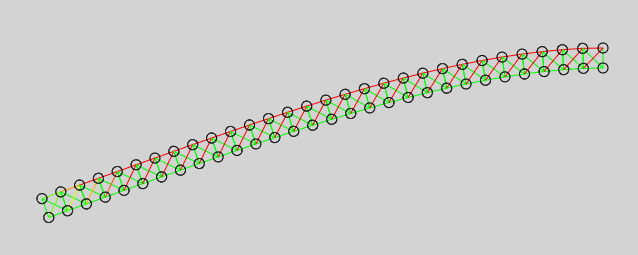
\includegraphics[width=11cm]{rgc compliance.png}
\caption{Compliance of a theoretically rigid beam with $s = 1$}
\label{fig:figure}
\end{figure} 
It was observed that the $constraintSolvingIterationNumber$ $\text{(Algorithm 3)}$ significantly affects the system’s stiffness. The reason for this behaviour is due to the repeated decrease of the truncation error $O(\Delta q_j^{2})$ $\text{(Equation 28)}$ as $\Delta q_j$ is lowered every iteration.
\begin{figure}[H]
\centering
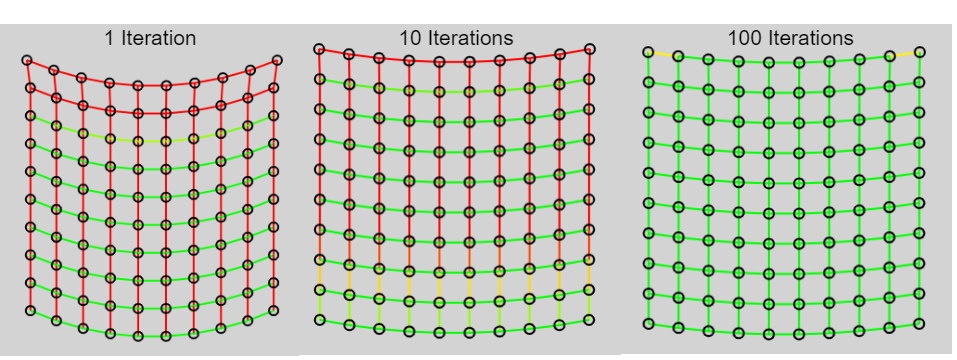
\includegraphics[width=12cm]{rgc iteration.png}
\caption{The stiffness increases in a cloth simulation as constraintSolvingIterationNumber increases}
\label{fig:figure}
\end{figure} 
\noindent To resolve the lower stiffness for smaller values of $constraintSolvingIterationNumber$, the stiffness factor, $s$, can be increased as compensation. However, the exact scaling will need to be experimentally determined. Moreover, RGCs also exhibit different stiffness responses with different $\Delta t$ $\text{(Figure 15)}$. 
\begin{figure}[H]
\centering
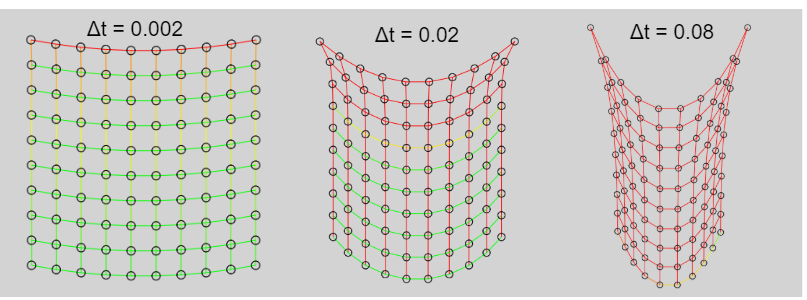
\includegraphics[width=11cm]{rgc timestep.png}
\caption{The stiffness decrease in a cloth simulation as the timestep increases}
\label{fig:figure}
\end{figure} 
\noindent The system is less stiff as the $\Delta t$ increases. The reason of this effect is due to the external forces acting on each RGC (Forces are not internal as $\Delta t$ is not in Equation 38). In the specific example shown in Figure 15, the particles are acted on by a gravity force. To apply the gravity force, it must be discretized by $\Delta t$ ($\text{Equation 3}$). Larger values of $\Delta t$ impart a larger displacement. Larger external displacements cause larger $\Delta q_j$ compensation which increases the truncation error of the constraint $\text{(Equation 28)}$, hence lowering the perceived stiffness.

The inconsistent stiffness values undermine RGC's credibility as a rigorous physics simulator, but as long as the initial parameters remain consistent, it can still simulate visually realistic effects $\text{(Macklin)}$.

\subsubsection{Constraint Convergence and Energy Conservation}
 \hspace{\parindent} The conditions for the convergence and stability of RGCs coincide with the conditions for PCs. Comparatively, RGCs are more stable because they are a position-based method. But also as a result, RGCs neglect energy conservation. Moreover, the constraint error - which is effected by $\Delta q_j$ $\text{(Equation 28)}$ -  results in inconsistent system energies.
 
 It is observed that the energy loss phenomenon is more apparent when the\\
 $constraintSolvingIterationNumber$, $csn$, is higher. Increasing $csn$ is equivalent to accelerating the time to $csn \cdot \Delta t$. Therefore, the original error from 1 iteration will be stacked $csn$ times, resulting in greater energy loss. A larger $\Delta t$ also increases $\Delta q_j$ and results in more energy instability. This phenomenon is supported with a graphical analysis of an oscillating RGC pendulum system $\text{(Raw data available in Appendix A)}$.
\begin{figure}[H]
\centering
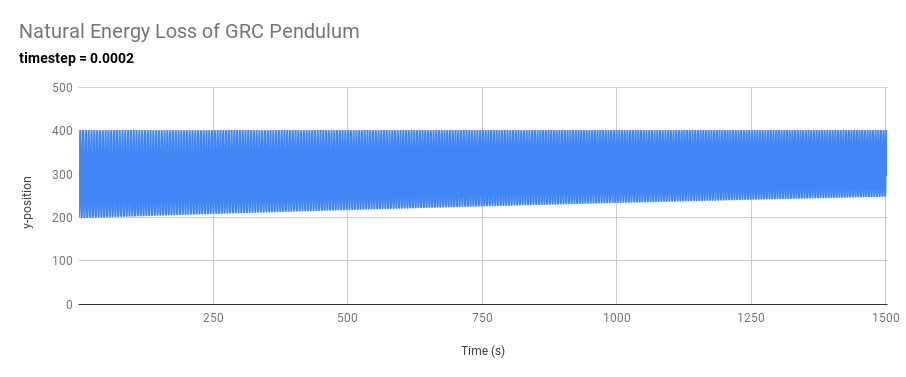
\includegraphics[width=15.5cm]{grc pendulum 0.0002.png}
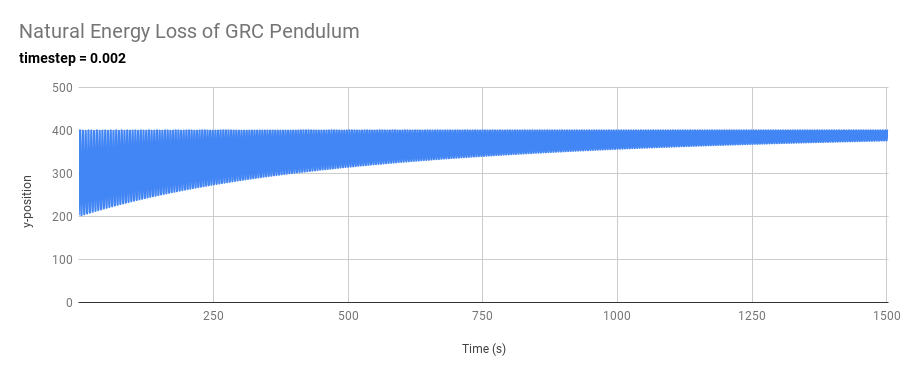
\includegraphics[width=15.5cm]{grc pendulum 0.002.png}
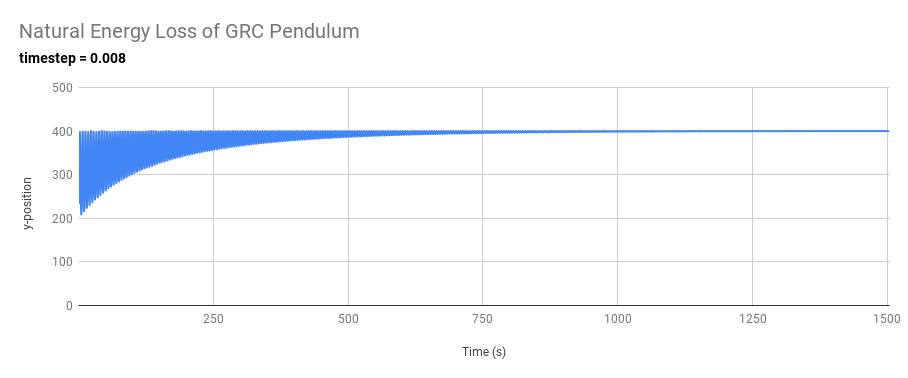
\includegraphics[width=15.5cm]{grc pendulum 0.008.png}
\caption{y-position vs time graphs of RGC pendulum systems at different $\Delta t$}
\label{fig:figure}
\end{figure} 
\noindent System convergence depends on the Gauss-Seidel solver ($\text{Section 2.2.3}$), meaning higher values of $constraintSolvingIterationNumber$ result in faster convergence. Conversely, divergence can occur when the truncation error overshoots. Overshoot typically occurs when a sudden external force is applied to the system (collisions and user interactions). Stiffer systems with a larger $s$ are also more likely to overshoot and diverge. Similarly, systems are also more likely to diverge with larger values of $constraintSolvingIterationNumber$ as any overshoot will also be magnified $constraintSolvingIterationNumber$ times. Typically, the truncation error is more likely to cause undershoot, resulting in energy loss and convergence. In general, RGCs are mainly effected by divergence when there are rapid, sudden, or large movements.

\section{Conclusion}
\hspace{\parindent}With the improvement of computing technology, physical modelling has become a much more prevalent field of study. Computational modelling has opened a new perspective of how humans perceive the world. This paper discussed modelling techniques of particle-based systems with penalty $\text{(Equation 23)}$ and relaxed geometric constraints $\text{(Equation 38)}$. Additionally, the system also utilizes a predictor-corrector semi-implicit Euler integration algorithm with a local iterative solver $\text{(Algorithm 1)}$. To summarize, penalty constraints are force-based, energy conservative, and easily damped. Unfortunately, they also diverge quickly for rigid systems and often require a large amounts of force penalties. On the other hand, RGCs are easier to implement, more versatile, and can be more rigid. Disadvantages of RGCs include their $\Delta t$ dependence and lack of energy conservation. As the final verdict, RGCs are generally a better choice for modelling non-rigorous physics simulations. Whereas PCs are suitable for modelling non-rigid physically accurate systems. 

Only a small sample of the existing modelling techniques was discussed. With all the different integration algorithms, system solvers, and constraint algorithms, the possible combinations are endless. A majority of the described techniques are rapidly evolving as technology and understanding improves with time. In the modern world where physical modelling can encompass video game physics to highly technical engineering analysis, the field of computational mathematics is a relevant and imperative subject. Some applications of RGCs and PCs include structural modelling, stress analysis, animation, and interactive surgical simulations $\text{(Bender)}$. Further study of this area is recommended due to the limitations imposed on this paper. Consequently, this paper was unable to analyze a major method in the literature using differential maintained constraints $\text{(Witkin)}$. Perhaps extensions to higher dimensions along with specific analyses of different use cases would  provide a more comprehensive understanding of the subject. But arguably, the most important step is to continuously experiment with new methods and resolve the current issues, elevating computer modelling to the next stage.
\clearpage

\section{Bibliography}
%TC:ignore
\noindent
\vspace{-2em}
\setlength{\parindent}{-0.5in}
\setlength{\leftskip}{0.5in}
%\setlength{\parskip}{15pt}

Adams, Douglas E. “ME 563 Mechanical Vibrations Lecture \#20 - Purdue University.” ME 563 Mechanical Vibrations Lecture \#20, Purdue University, 2010, engineering.purdue.edu/~deadams/ME563/lecture2010.pdf. Accessed Nov 28, 2021.

Bender, Jan, et al. “A Survey on Position-Based Simulation Methods in Computer Graphics.” Computer Graphics Forum, vol. 33, no. 6, 2014, pp. 228–251., doi:10.1111/cgf.12346.

Clavet, Simon, et al. “Particle-Based Viscoelastic Fluid Simulation.” Proceedings of the 2005 ACM SIGGRAPH/Eurographics Symposium on Computer Animation - SCA '05, 2005, doi:10.1145/1073368.1073400.

Fitzpatrick , Richard. Numerical Errors, 29 Mar. 2006, farside.ph.utexas.edu/teaching/ 329/lectures/node33.html. Accessed Jun 20, 2021.

Goldstein, Herbert, et al. Classical Mechanics. Pearson, 2014. 

Gutiérrez, José Manuel, et al. “The ‘Gauss-Seidelization’ of Iterative Methods for Solving Nonlinear Equations in the Complex Plane.” Applied Mathematics and Computation, vol. 218, no. 6, 2011, pp. 2467–2479., doi:10.1016/j.amc.2011.07.061. 

Jakobsen, Thomas. (2001). Advanced character physics. In-Game Developers Conference Proceedings. 

Liu, Mingzhu, et al. “Convergence and Stability of the Semi-Implicit Euler Method for a Linear Stochastic Differential Delay Equation.” Journal of Computational and Applied Mathematics, vol. 170, no. 2, 2004, pp. 255–268., doi:10.1016/j.cam.2004.01.040. 

Macklin, Miles, et al. “XPBD.” Proceedings of the 9th International Conference on Motion in Games, 2016, doi:10.1145/2994258.2994272. 

Müller, Matthias, et al. "Position based dynamics." Journal of Visual Communication and Image Representation 18.2 (2007): 109-118.

Nealen, Andrew, et al. “Physically Based Deformable Models in Computer Graphics.” Computer Graphics Forum, vol. 25, no. 4, 2006, pp. 809–836., doi:10.1111/j.1467-8659.2006.01000.x.  

Spiegel, Murray R. Schaum's Outline of Theory and Problems of Theoretical Mechanics with an Introduction to Lagrange's Equations and Hamiltonian Theory. Schaum Publishing Co., 1994. 

Strang, Gilbert. Introduction to Linear Algebra. Wellesley-Cambridge Press, 2016. 

Witkin, Andrew, and David Baraff. Physically Based Modeling, Siggraph '97, 1997, www .cs.cmu.edu/~baraff/sigcourse/, Accessed 10 April 2021. 

\clearpage
\indent
\vspace{-2em}
\setlength{\parindent}{-0.5in}
\setlength{\leftskip}{0cm}

\section{Appendix A: Additional Resources}
All demonstrations are accessible on a modern computer browser (Google Chrome, Microsoft Edge, Brave, Firefox, Safari is untested). The demonstrations implements the stretch constraint for both RGCs and PCs, where $C(x_{1},x_{2}) = |x_{1}-x_{2}|-r$.\\

\noindent Main webpage for all demonstrations and implementations: 
\url{https://onlinedocumentation.github.io/Math-EE/}\\

\noindent All Source Codes:  \url{https://github.com/onlineDocumentation/Math-EE} \\

\noindent Penalty Constraints demo: \url{https://onlinedocumentation.github.io/Math-EE/Math-EE-Penalty-Constraints/index.html} \\

\noindent Penalty Constraints Source Code: \url{https://github.com/onlineDocumentation/Math-EE/tree/main/Math-EE-Penalty-Constraints} \\

\noindent Relaxed Geometric Constraints demo: \url{https://onlinedocumentation.github.io/Math-EE/Math-EE-Relaxed-Geometric-Constraints/index.html}\\

\noindent Relaxed Geometric  Constraints Source Code: \url{https://github.com/onlineDocumentation/Math-EE/tree/main/Math-EE-Relaxed-Geometric-Constraints}\\

\noindent Raw Data for Pendulum Graphs: \url{https://onlinedocumentation.github.io/Math-EE/pendulumdata.html }

\clearpage

\section{Appendix B: Detailed Calculations}
\subsection{Detailed PC Stretch Constraint Derivation}
\subsubsection{Part 1: No damping}

Given $C_j(x_{1},x_{2}) = |x_{1}-x_{2}|-r= \sqrt{(x_{1}-x_{2}) \cdot (x_{1}-x_{2})} - r$
$$F_{x_{1}}=\frac{\partial E}{\partial x_{1}}=-kC_j\cdot \frac{\partial C_j}{\partial x_{1}}$$
$$F_{x_{2}}=\frac{\partial E}{\partial x_{2}}=-kC_j\cdot \frac{\partial C_j}{\partial x_{2}}.$$
First, solving for $\frac{\partial C_j}{\partial x_{1}}$ by using the chain rule then product rule
$$\frac{\partial C_j}{\partial x_{1}} = \frac{1}{2 \sqrt{(x_{1}-x_{2}) \cdot (x_{1}-x_{2})}} ((1-0)(x_{1}-x_{2}) + (x_{1}-x_{2})(1-0))$$
$$= \frac{2(x_{1}-x_{2})}{2 \sqrt{(x_{1}-x_{2}) \cdot (x_{1}-x_{2})}}$$
$$=\frac{x_{1}-x_{2}}{|x_{1}-x_{2}|}.$$
Combining yields,
$$F_{x_{1}} = -k( |x_{1}-x_{2}|-r) \cdot \frac{x_{1}-x_{2}}{|x_{1}-x_{2}|}$$
Similarly,
$$\frac{\partial C}{\partial x_{2}} = \frac{1}{2 \sqrt{(x_{1}-x_{2}) \cdot (x_{1}-x_{2})}} ((0 -1)(x_{1}-x_{2}) + (x_{1}-x_{2})(0 - 1))$$ $$ =- \frac{x_{1}-x_{2}}{|x_{1}-x_{2}|}$$
$$F_{x_{2}} = k( |x_{1}-x_{2}|-r) \cdot \frac{x_{1}-x_{2}}{|x_{1}-x_{2}|}.$$
\subsubsection{Part 2: With damping}
Penalty force discretization with damping, extending from Section 7.1.1
$$\Delta x_{i} = w_{i}(-kC_j - \mu \dot{C_j}) \cdot \frac{\partial C_j}{\partial x_{i}} \Delta t^{2}$$
First calculating $\dot{C_j}$, where
$$\dot{C_j} = \frac{d}{dt}(\sqrt{(x_{1}-x_{2}) \cdot (x_{1}-x_{2})} - r)$$
$$= \frac{1}{2 \sqrt{(x_{1}-x_{2}) \cdot (x_{1}-x_{2})}} \left[ \left( \frac{dx_{1}}{dt} - \frac{dx_{2}}{dt} \right)\cdot (x_{1} - x_{2}) + (x_{1} - x_{2})\cdot \left(\frac{dx_{1}}{dt} - \frac{dx_{2}}{dt}\right) \right] .$$
Of which $\frac{dx_{i}}{dt}$ is the velocity of $x_{i}$, $v_{i}$. Replacing results in, 
$$= \frac{2 (v_{1} - v_{2})\cdot (x_{1} - x_{2})}{2 \sqrt{(x_{1}-x_{2}) \cdot (x_{1}-x_{2})}}$$
$$= \frac{(v_{1} - v_{2}) \cdot (x_{1} - x_{2})}{|x_{1}-x_{2}|}.$$
Combining all the components from part 1 and part 2 give, 
$$\Delta x_{1} = w_{1}\left(-k(|x_{1}-x_{2}|-r) - \mu \frac{(v_{1} - v_{2}) \cdot (x_{1} - x_{2})}{|x_{1}-x_{2}|}\right) \cdot \frac{x_{1}-x_{2}}{|x_{1}-x_{2}|} \Delta t^{2}$$
$$\Delta x_{2} = -w_{2}\left(-k(|x_{1}-x_{2}|-r) - \mu \frac{(v_{1} - v_{2}) \cdot (x_{1} - x_{2})}{|x_{1}-x_{2}|}\right) \cdot \frac{x_{1}-x_{2}}{|x_{1}-x_{2}|} \Delta t^{2}.$$

\subsection{Detailed RGC Stretch Constraint Derivation}
Given $C_j(x_{1},x_{2}) = |x_{1}-x_{2}|-r = \sqrt{(x_{1}-x_{2}) \cdot (x_{1}-x_{2})} - r $
$$ \Delta q_{j,i} = -w_{j,i} s_j \frac{C_j(q_j)}{\sum\limits^{n}_{u} w_{j,u}[ \nabla_{q_{j,k}}C_j(q_j) \cdot \nabla_{q_{j,k}}C_j(q_j)]} \nabla_{q_{j,i}}C_j(q_j).$$
$q_j = [x_1\;\;x_2]^T$, therefore $q_{j,1} = x_1$ and $q_{j,2} = x_2$. Using the above equation yields, 
$$\Delta x_{1} = -w_{1} s \frac{C_j(q_j)}{\sum\limits^{n}_{u} w_{j,u}[ \nabla_{x_{u}}C_j(q_j) \cdot \nabla_{q_{j,u}}C_j(q_j)]}\nabla_{x_{1}}C_j(q_j)$$ 
 $$\Delta x_{2} = -w_{2} s \frac{C_j(q_j)}{\sum\limits^{n}_{u} w_{j,u}[ \nabla_{q_{j,u}}C_j(q_j) \cdot \nabla_{q_{j,u}}C_j(q_j)]}\nabla_{x_{2}}C_j(q_j).$$
Next, each section is solved by steps. First, $\nabla_{x_{i}}C_j(q_j)$ is calculated for $x_1$ and $x_2$,
$$ \nabla_{q_{j,1}}C_j(q_j) = 1 - 0 = 1$$ 
$$\nabla_{q_{j,2}}C_j(q_j) = 0 - 1 = -1.$$
Then, the denominator $\sum\limits^{n}_{u} w_{j,u}[ \nabla_{x_{u}}C_j(q_j) \cdot \nabla_{q_{j,u}}C_j(q_j)]$ is simplified to, 
$$\sum\limits^{n}_{u} w_{j,u}[ \nabla_{x_{u}}C_j(q_j) \cdot \nabla_{q_{j,u}}C_j(q_j)] = w_{1} \cdot 1 + w_{2} \cdot 1 = w_{1} + w_{2}. $$
Lastly, substituting each component yields,
$$\Delta x_{1} = -s\frac{w_{1}}{w_{1}+w_{2}}(|x_{1} - x_{2}|-r) \frac{x_{1} - x_{2}}{|x_{1} - x_{2}|}$$ 
$$\Delta x_{2} = s\frac{w_{2}}{w_{1}+w_{2}}(|x_{1} - x_{2}|-r) \frac{x_{1} - x_{2}}{|x_{1} - x_{2}|}.$$
%TC:endignore

%\section{Appendix C}

%\clearpage

\end{document}
